% This file was created with tikzplotlib v0.10.1.
\begin{tikzpicture}

\definecolor{darkorange25512714}{RGB}{255,127,14}
\definecolor{darkslategray38}{RGB}{38,38,38}
\definecolor{forestgreen4416044}{RGB}{44,160,44}
\definecolor{lightgray204}{RGB}{204,204,204}
\definecolor{steelblue31119180}{RGB}{31,119,180}

\begin{axis}[
axis line style={lightgray204},
height=0.35\textheight,
legend cell align={left},
legend style={
  fill opacity=0.8,
  draw opacity=1,
  text opacity=1,
  at={(0.97,0.03)},
  anchor=south east,
  draw=none
},
log basis y={10},
tick align=outside,
tick pos=left,
title={Iterations per second scaling with number of threads},
width=\textwidth,
x grid style={lightgray204},
xlabel=\textcolor{darkslategray38}{Thread count},
xmajorgrids,
xmin=-0.55, xmax=33.55,
xtick style={color=darkslategray38},
y grid style={lightgray204},
ylabel=\textcolor{darkslategray38}{Iterations per second},
ymajorgrids,
ymin=10.1142300373004, ymax=126.127813659134,
ymode=log,
ytick style={color=darkslategray38},
ytick={1,10,100,1000,10000},
]
\path [draw=black, semithick]
(axis cs:1,11.3434579426129)
--(axis cs:1,11.4169387954404);

\path [draw=black, semithick]
(axis cs:2,18.9235958444644)
--(axis cs:2,19.2150275724177);

\path [draw=black, semithick]
(axis cs:4,35.8578390024344)
--(axis cs:4,37.0411514425839);

\path [draw=black, semithick]
(axis cs:8,53.113113274484)
--(axis cs:8,62.8447872008034);

\path [draw=black, semithick]
(axis cs:16,64.4104664378055)
--(axis cs:16,87.675718809926);

\path [draw=black, semithick]
(axis cs:32,63.8600841437675)
--(axis cs:32,90.7974484257651);

\path [draw=black, semithick]
(axis cs:1,19.8863255514302)
--(axis cs:1,20.1994580254242);

\path [draw=black, semithick]
(axis cs:2,37.4057343839802)
--(axis cs:2,39.0663338107513);

\path [draw=black, semithick]
(axis cs:4,64.8449029912199)
--(axis cs:4,69.9016522130963);

\path [draw=black, semithick]
(axis cs:8,96.1864991499843)
--(axis cs:8,102.997087166422);

\path [draw=black, semithick]
(axis cs:16,104.453066363991)
--(axis cs:16,112.460038896781);

\path [draw=black, semithick]
(axis cs:32,87.3535081696029)
--(axis cs:32,100.511890029895);

\path [draw=black, semithick]
(axis cs:1,19.9503529850887)
--(axis cs:1,20.6670312553662);

\path [draw=black, semithick]
(axis cs:2,36.7496359591628)
--(axis cs:2,38.8018901816652);

\path [draw=black, semithick]
(axis cs:4,63.4743409940291)
--(axis cs:4,71.4238109012899);

\path [draw=black, semithick]
(axis cs:8,98.2238726836014)
--(axis cs:8,101.948275363719);

\path [draw=black, semithick]
(axis cs:16,105.972254715636)
--(axis cs:16,111.183011299564);

\path [draw=black, semithick]
(axis cs:32,87.3092415333317)
--(axis cs:32,98.9070300444787);

\addplot [semithick, steelblue31119180, mark=x, mark size=3, mark options={solid}]
table {%
1 11.3801984786987
2 19.0693092346191
4 36.4494972229004
8 57.9789543151855
16 76.0430908203125
32 77.3287658691406
};
\addlegendentry{Rust, problem size=128}
\addplot [semithick, darkorange25512714, mark=x, mark size=3, mark options={solid}]
table {%
1 20.0428905487061
2 38.2360305786133
4 67.3732681274414
8 99.5917892456055
16 108.456520080566
32 93.9327011108398
};
\addlegendentry{C++, problem size=128}
\addplot [semithick, forestgreen4416044, mark=x, mark size=3, mark options={solid}]
table {%
1 20.3086967468262
2 37.7757682800293
4 67.4490814208984
8 100.086059570312
16 108.57763671875
32 93.108154296875
};
\addlegendentry{FORTRAN, problem size=128}
\end{axis}

\end{tikzpicture}
